%%%%%%%%%%%%%%%%%%%%%%%%%%%%%%%%%%%%%%%%%%%%%%%%%%%%%%%%%%%%%%%%%%%%%%%%%%%%%%%

\subsection{Used Technologies}
\label{sec:UsedTechnologies}

This section lists all technologies and libraries used in \textan{}.

\paragraph{Apache CXF\footnote{\url{http://cxf.apache.org/}}}
Apache CXF is an open-source Web services framework. CXF implements the JAX-WS
standard APIs, is configurable through Spring and can be embedded into Jetty,
Tomcat or other servlet containers.

\paragraph{ControlsFX\footnote{\url{http://fxexperience.com/controlsfx/}}}
ControlsFX is a Java8 open source library aiming at enhancing the programming
experience with standard JavaFX. It provides wide selection of new and improved
components to make everyday use of JavaFX even easier.

\paragraph{Hibernate ORM\footnote{\url{http://hibernate.org/orm/}}}
Hibernate ORM (Hibernate in short) is an object-relational mapping library for
Java language, providing a framework for mapping an object-oriented domain
model to a traditional relational database. Hibernate solves object-relational
im\-pedance mismatch problems by replacing direct persistence-related database
accesses with high-level object handling functions.

\paragraph{Hibernate Search\footnote{\url{http://hibernate.org/search/}}}
Hibernate Search is a library (or Hibernate ORM extension), which integrates
the full text library functionality from Apache Lucene in the Hibernate and
JPA model. It offers full-text search support for objects stored by Hibernate
ORM, Infinispan and other sources. Think of it as Google\texttrademark{} for
entities: search words with text, order results by relevance and find by
approximation (fuzzy search).

\paragraph{JCommander\footnote{\url{http://jcommander.org/}}}
JCommander is a very small Java framework that makes it trivial to parse command
line parameters.

\paragraph{Jetty\footnote{\url{http://www.eclipse.org/jetty/}}}
Jetty is a pure Java-based HTTP (Web) server and Java Servlet container. It can
be embedded into other applications through Jetty API.

\paragraph{JUNG\footnote{\url{http://jung.sourceforge.net/}}}
JUNG (Java Universal Network/Graph Framework) is an older Java library for
displaying graphs for Swing framework, still widely used in Java world, well documented and easily extensible.
\comment[Petr]{Tam}{Older than what? Or just old?}

\paragraph{JFXtras\footnote{\url{http://jfxtras.org/}}}
JFXtras is another JavaFX8 enhancing project providing components that
most Java developers need in daily work, but they are currently missing
from JavaFX.

\paragraph{MorphoDiTa\footnote{\url{http://ufal.mff.cuni.cz/morphodita}}}
Morphological Dictionary and Tagger is an open-source tool for morphological
analysis of natural language texts. It performs morphological analysis, 
morphological generation, tagging and tokenization and is distributed as
a standalone tool or a library, along with trained linguistic models. In
the Czech language, MorphoDiTa achieves state-of-the-art results with 
a throughput around 10-200K words per second. MorphoDiTa is a free software
under LGPL license and the linguistic models are free for non-commercial use
and distributed under CC BY-NC-SA license, although for some models the original
data used to create the model may impose additional licensing conditions.
\comment[Petr]{Tam}{This paragraph is flawless. Do we need a quotation here? (maybe other tools as well)}

\paragraph{NameTag\footnote{\url{http://ufal.mff.cuni.cz/nametag}}}
NameTag is an open-source tool for named entity recognition (NER). NameTag 
identifies proper names in text and classifies them into predefined categories,
such as names of persons, locations, organizations, etc. NameTag is distributed
as a standalone tool or a library, along with trained linguistic models.
In the Czech language, NameTag achieves state-of-the-art performance
(Straková et al. 2013). NameTag is a free software under LGPL license and the 
linguistic models are free for non-commercial use and distributed under CC 
BY-NC-SA license, although for some models the original data used to create
the model may impose additional licensing conditions.
\comment[Petr]{Tam}{This paragraph is flawless. Do we need a quotation here? (maybe other tools as well)}


\paragraph{PretopoLib\footnote{\url{http://pretopolib.complexica.net/}}}
PretopoLib is a JAVA library based on pretopology. It provides the mathematical 
theory which supports
analysis, modelling and simulation in several domains: human and social sciences,
game theory, graph theory extension, networks and discrete spaces.
\comment[Petr]{Tam}{Approved?}

\paragraph{SLF4J \& Logback\footnote{\url{http://www.slf4j.org/}, \url{http://logback.qos.ch/}}}
Simple Logging Facade for Java (SLF4J) provides a Java logging API by means
of a simple facade pattern. The underlying logging backend is determined
at runtime by adding the desired binding to the classpath and may be
java.util.logging, log4j or logback.

\paragraph{Spring Framework\footnote{\url{http://projects.spring.io/spring-framework/}}}
The Spring Framework is an open source application framework and inversion
of control container for the Java platform. The framework's core features
can be used by any Java application, but there are extensions for building
web applications on top of the Java EE platform.

\comment{Ondrej}{Spring should be first in the list, other items mention it.}

\paragraph{WEKA\footnote{\url{http://www.cs.waikato.ac.nz/ml/weka/}}}
Weka is a collection of machine learning algorithms for data mining tasks.
The algorithms can either be applied directly to a dataset or called from your
own Java code. Weka contains tools for data pre-processing, classification,
regression, clustering, association rules, and visualization. It is also
well-suited for developing new machine learning schemes.

\paragraph{} For more information about libraries and their usage in client see
\ref{ssec:UsedLibraries}.

\subsection{Decisions}

\comment{Petr}{Why we used technologies mentioned above.}

\comment[Venca]{Petr}{\huge{Write all database related decisions!}}

\subsection{Mockup Screens}

This section contains mockup screens for the most important windows in \textan{}
client.

\begin{figure}[!htb]
        \centering
        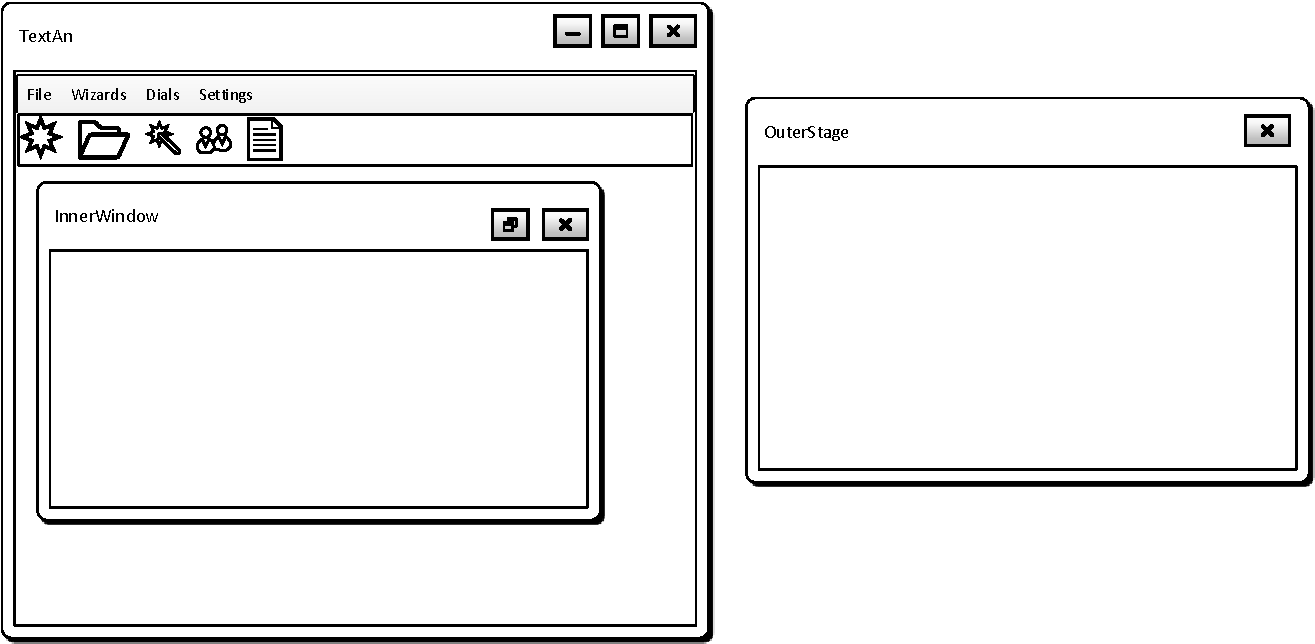
\includegraphics[width=\textwidth]{Images/MockupMainWindow}
        \caption{Mockup screen of the main window.}
        \label{fig:MockupMainWindow}
\end{figure}

\comment[Adam]{Adam}{Add more mockup screens.}